\begin{title}
  Практические задания в gap
\end{title}

\begin{title}
  Задание №1
\end{title}

\emph{1) Нахождение примитивного элемента p(простое число) в поле $GF(p)$.}\\
Определим для начала простое число:\\

\begin{center}
  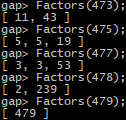
\includegraphics[width = 3cm]{Prostoe}
\end{center}

Так как p = 473, то в поле $GF(473)$ определим примитивный элемент:\\

\begin{center}
  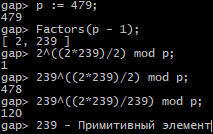
\includegraphics[width = 4cm]{Primitiv}
\end{center}

\emph {2) Решить систему уравнений по модулю $p$ в поле $GF(p)$}\\

\begin{equation*}
 \begin{cases}
    2x + 3y - 4z = 5\\
    4x - 5y + 5z = 6\\
    5x + 2y - z = 4
 \end{cases}
\end{equation*}

\begin{center}
  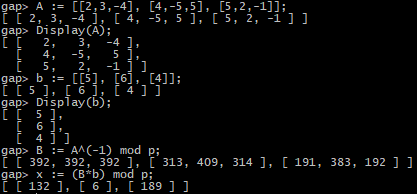
\includegraphics[width = 7cm]{Matriza}
\end{center}

\emph {3) Найти обратимый элемент по модулю $p$ в поле $GF(p)$}\\
$p = 473 \Rightarrow GF(473)$\\

\begin{center}
  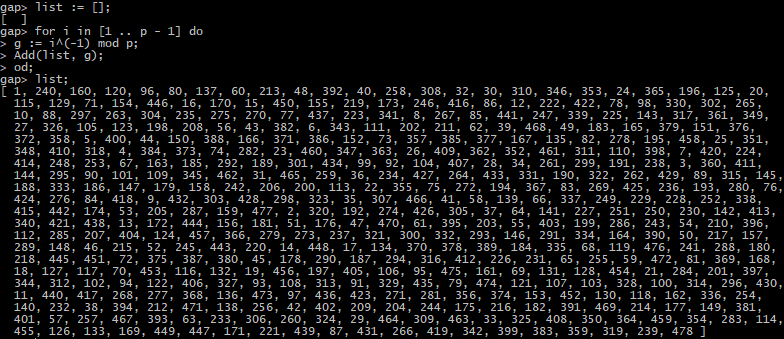
\includegraphics[width = 12cm]{Obrat}
\end{center}

\emph {4) Решение квадратного уравнения по модулю $p$ в поле $GF(p)$}\\
$p = 473 \Rightarrow GF(473)$\\
Уравнение: $2x^2 -4x + 2017 = 0$\\

\begin{center}
  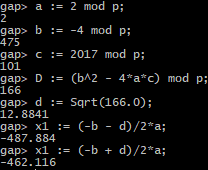
\includegraphics[width = 4cm]{Kvadrat}
\end{center}

\emph {5) ФИО}\\
Имя = 6, Фамилия = 6, Отчество = 7\\

\begin{center}
  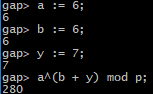
\includegraphics[width = 3cm]{FIO}
\end{center}

\begin{title}
  Задание №2
\end{title}

\emph {1) Зашифровать свое имя по алгоритму RSA}\\
Даниил = 40128810\\

$p = 3343$ и $q = 31573$ - простые числа\\
\[n = p*q = 105548539\]
\[f(n) = (p - 1)(q - 1) = 105513624\]
Выберем открытую экспоненту $e = 73$
$(e, n) = (79 , 105548539)$ - открытый ключ\\
Закрытая экспонента равна $e^{-1} mod f(n) = 13008529$\\
$(13008529, 105548539)$ - закрытый ключ\\
Результат шифрования и дешифрования представлен ниже:\\

\begin{center}
  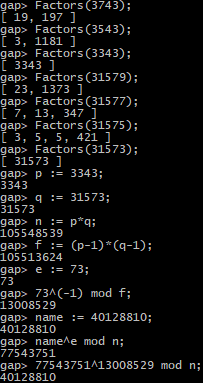
\includegraphics[width = 4cm]{Name}
\end{center}

\emph {2) Найти простое шестнадцатизначное число}\\

\begin{center}
  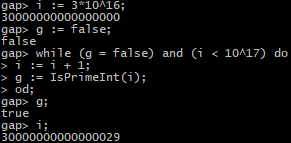
\includegraphics[width = 6cm]{Prost16}
\end{center}

{\bf \emph {III) Линейный регистр сдвига с обратной связью}}\\
Допустим, что рекурентная последовательность задается характеристическим
многочленом
$x^4 + x^3 + x^2 + 1$.\\
Тогда функция обратной связи имеет вид $f = b_4 \oplus b_3 \oplus b_2$.\\
Допустим, что начальным состоянием регистра сдвига являестся последовательность
$[b_1, b_2, b_3, b_4] = [0, 1, 1, 1]$.\\

\begin{table}[h]
  \begin{center}
    \begin{tabular}{|c|c|c|c|}
      \hline
      Номер состояния & $b_1, b_2, b_3, b_4$ & $f =  b_4 \oplus b_3 \oplus b_1$
      & Генерируемы бит\\
      \hline
       0 & 0 1 1 1 & 1 & 1 \\
       \hline
       1 & 1 0 1 1 & 0 & 1 \\
       \hline
       2 & 0 1 0 1 & 0 & 1 \\
       \hline
       3 & 0 0 1 0 & 1 & 0\\
       \hline
       4 & 1 0 0 1 & 1 & 1\\
       \hline
       5 & 1 1 0 0 & 1 & 0\\
       \hline
       6 & 1 1 1 0 & 0 & 0\\
       \hline
       7 & 0 1 1 1 & 1 & 1\\
       \hline
    \end{tabular}
  \end{center}
\end{table}
То есть генерируемая последовательность имеет вид: $[1, 1, 1, 0, 1, 0, 0, 1,
\cdots]$ и ее период равен 7\\

\begin{title}
  Задание №3
\end{title}

Код для написан для решения задач типа
$$
\left\{
\begin{array}{lc}
  k_1 = b_1 & (mod ~ m_1) \\
  k_2 = b_2 & (mod ~ m_2) \\
  \ldots & \ldots \\
  k_i = b_i & (mod ~ m_i)
\end{array}
\right. ~~ i \ge 1
$$

\lstinputlisting{../gap/3.g}

Вывод программы
\begin{lstlisting}
size = 3
kx = [ 9, 8, 7 ]
free = [ 7, 8, 9 ]
module = [ 5, 7, 11 ]
kanon = [ 3, 1, 6 ]
solution = [ [ 3, 5 ], [ 1, 7 ], [ 10, 11 ] ]
commonSolution = [ 358, 385 ]
\end{lstlisting}

Уравнение
$$
\left\{
\begin{array}{l}
  9x = 7 ~ (mod ~ 5)\\
  8x = 8 ~ (mod ~ 7)\\
  7x = 9 ~ (mod ~ 11)
\end{array}
\right.
$$
Канонический вид
$$
\left\{
\begin{array}{l}
  x = 3 \\
  x = 1 \\
  x = 6
\end{array}
\right.
$$
Решение
$$
\left\{
\begin{array}{l}
  x = 3 + 5y \\
  y = 1 + 7z \\
  z = 10 + 11t \\
\end{array}
\right.
$$
Общее решение $x = 358$ (mod $385$) \\

Если руками руками тогда

1) решение первого уравнения

$x = 3 + 5y$

2) решение второго уравнения

$3 + 5y = 1$

$y = -\frac{2}{5}$

$y = 1 ~ mod ~ 7 ~ \Rightarrow ~ y = 1 + 7z$

3) решение третьего уравнения

$x = 3 + 5(1 + 7z) = 8 + 35z = 6$

$z = -\frac{2}{35}$

$z = 10 ~ mod ~ 11 ~ \Rightarrow ~ z = 10 + 11t$

4) Общее решение

$x = 8 + 35(10 + 11t) = 358 + 385t$

$x = 358 ~ (mod ~ 385)$

\begin{title}
  Задание №4
\end{title}
\emph {1) По рекурентной последовательности написать ее матрицу
$A$ и зарактеристический многочлен}\\
Простое число $p = 473 \Rightarrow GF(473)$\\
Вектор инициализации: $\bar{S_0} = (150, 45, 220, 55)$ . Кратность $k = 4$.\\
Рекурентная последовательность имеет вид:
\[S_{n+4} = 150S_{n+3} + 45S_{n+2} + 220S_{n+1} + 55S_n\]
Матрица A имеет вид:\\

$$
A =
\left(
\begin{array}{lccr}
  0 & 0 & 0 & 150\\
  1 & 0 & 0 & 45\\
  0 & 1 & 0 & 220\\
  1 & 0 & 1 & 55
\end{array}
\right)
$$

Характеристический многочлен:
\[x^4 = 150x^3 + 45x^2 + 220x + 55\]

\emph {2) Найти корни характеристического многочлена, которые лежат в поле
$GF(p)$}\\
\[x^4 = 150x^3 + 45x^2 + 220x + 55 = (x + 314)(x + 156)(x + 150)(x + 27)\]
Корни по модулю: $x_1 = 165, x_2 = 323, x_3 = 329, x_4 = 470$\\

\emph {3) Найти явную форму этого многочлена.}
\begin{equation*}
 \begin{cases}
    \beta_1 + \beta_2 + \beta_3 + \beta_4 = 150\\
    165\beta_1 + 323\beta_2  + 329\beta_3 + 470\beta_4 = 45\\
    401\beta_1 +386 \beta_2 + 466\beta_3 + 81\beta_4 = 220\\
    63\beta_1 + 138\beta_2 + 34\beta_3 + 229\beta_4 = 55
 \end{cases}
\end{equation*}

\begin{center}
  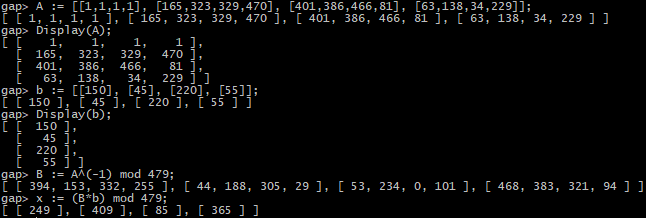
\includegraphics[width = 10cm]{4N}\\
  Решение методом Крамера
\end{center}

\begin{equation*}
 \begin{cases}
    \beta_1 = 249\\
    \beta_2 = 409\\
    \beta_3 = 85\\
    \beta_4 = 365
 \end{cases}
\end{equation*}

\emph {4) Явно вычислить последовательность, найти ее период для импульсной
функции}\\
\[S_n = 249\alpha_{1}^{n} + 409\alpha_{2}^{n} + 85\alpha_{3}^{n} +
365\alpha_{4}^{n}\]
Период последовательности не больше чем 478\\

\begin{center}
  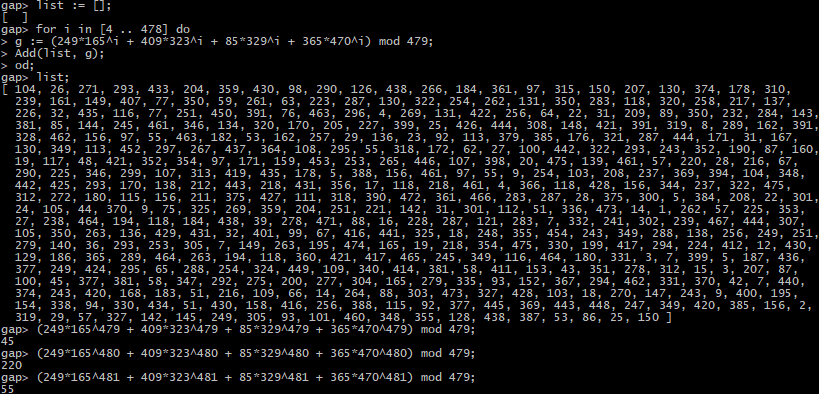
\includegraphics[width = 14cm]{Period}\\
\end{center}

Период равен 478.